% !TeX spellcheck = en_GB

% v14

\documentclass{article}

\usepackage{fancyhdr}
\usepackage{titlesec}
\usepackage{titling}
\usepackage{extramarks}
\usepackage{lastpage}
\usepackage{libertine}
\usepackage{ifthen}
\usepackage[
	a4paper,
	total={135mm, 240mm},
	includehead,
	headsep=12mm,
	footskip=15mm
]{geometry}
\usepackage{amsmath}
\usepackage{amsthm}
\usepackage{amssymb}
\usepackage{mathtools}
\usepackage{graphicx}
\usepackage[figuresleft]{rotating}
\usepackage{color}
\usepackage[
	backend=biber,
	style=numeric,
	citestyle=authoryear,
	maxnames=10,
]{biblatex}
\usepackage{listings}
\usepackage{xparse}
\usepackage{multirow}
\usepackage{xcolor}
\usepackage{booktabs}
\usepackage{bookmark}
\usepackage{draftfigure}
\usepackage{bbm}
\usepackage{tabularx}
\usepackage{verbatim}
\usepackage[ruled, vlined]{algorithm2e}
\usepackage{doi}
\usepackage{hyperref}
\usepackage{placeins}
\usepackage{flafter}
\usepackage[title]{appendix}

\definecolor{blue}{HTML}{1f77b4}
\definecolor{orange}{HTML}{ff7f0e}
\definecolor{green}{HTML}{2ca02c}
\definecolor{red}{HTML}{d62728}
\definecolor{purple}{HTML}{9467bd}
\definecolor{brown}{HTML}{8c564b}

\addbibresource{mybib.bib}
\renewbibmacro{in:}{}

% Custom commands

\DeclarePairedDelimiter\abs{\lvert}{\rvert}
\DeclareMathOperator{\E}{E}
\DeclareMathOperator{\Var}{Var}
\newcommand{\R}{\mathbb{R}}
\newcommand{\Z}{\mathbb{Z}}
\newcommand{\N}{\mathbb{N}}
\newcommand{\dd}{{\rm d}}
\newcommand{\eps}{\varepsilon}

\newcommand{\st}{\textsuperscript{st}}
\newcommand{\nd}{\textsuperscript{nd}}
\newcommand{\rd}{\textsuperscript{rd}}
\renewcommand{\th}{\textsuperscript{th}}

\NewDocumentCommand{\codeword}{v}{%
	\texttt{\textcolor{blue}{#1}}%
}

\newtheorem{theorem}{Theorem}[section]
\newtheorem{lemma}[theorem]{Lemma}

\newcommand{\metro}[7]{
	\begin{tabularx}{\linewidth}{@{}Xl@{}}
		\toprule[0.1em]
		Proposal distributions &#1\\
		Initialisation &#2\\
		Sample size &#3\\
		\midrule[0.1em]
		\raisebox{-10mm}{Traceplots} &\raisebox{%
				3mm - \totalheight}{%
				\includegraphics[width=0.8\linewidth]{#4}}\\
		\raisebox{-8mm}{Histograms} &\raisebox{%
			3mm - \totalheight}{%
			\includegraphics[width=0.8\linewidth]{#5}}\\
		Acceptance rates &#6\\
		%Means&#7\\ 
		\bottomrule[0.1em]
	\end{tabularx}
}

\newcommand{\metrogroup}[4]{
	\begin{table*}
		\caption{Metropolis-Hastings algorithm for #2
			with $k = 3$ and #4 copula prior.}
		\centering
		\renewcommand{\arraystretch}{1.2}
		\input{latex-bits/#1-3-#3-prior.txt}
		\label{table:#1-#3-1}
	\end{table*}
	
	\begin{table*}
		\caption{Metropolis algorithm for #2
			with $k = 3$ and #4 copula posterior.}
		\centering
		\renewcommand{\arraystretch}{1.2}
		\input{latex-bits/#1-3-#3-post.txt}
	\end{table*}

	\begin{table*}
		\caption{Metropolis-Hastings algorithm for #2
			with $k = 2$ and #4 copula posterior.}
		\centering
		\renewcommand{\arraystretch}{1.2}
		\input{latex-bits/#1-2-#3-post.txt}
		\label{table:#1-#3-2}
	\end{table*}
}


\newcommand{\metroall}[2]{
	\metrogroup{#1}{#2}{i}{independent}
	\metrogroup{#1}{#2}{me}{maximum entropy}
}

\newcommand{\marginals}[6]{
	\begin{figure}
		\centering
		\includegraphics[%
						width=\linewidth]{%
						plots/#1-#3-uni-0-marg}
		\includegraphics[%
						width=\linewidth]{%
						plots/#1-#3-uni-1-marg}
		\includegraphics[%
						width=\linewidth]{%
						plots/#1-#3-uni-2-marg}
		\caption{Prior (dashed) and posterior (solid) marginals of
			$(#4, #5, #6)$, for priors with
			$k = 3$ and independent copula \textbf{\color{blue}{(blue)}},
			$k = 2$ and independent copula \textbf{\color{green}{(green)}},
			$k = 3$ and maximum entropy copula
			\textbf{\color{orange}{(orange)}}, and
			$k = 2$ and maximum entropy copula \textbf{\color{red}{(red)}}
			for #2.}
		\label{table:#1-#3-uni-marg}
	\end{figure}
}

\newcommand{\allmarginals}[2]{
	\marginals{#1}{#2}{theta}{\mu}{\log\sigma}{\xi}
	\marginals{#1}{#2}{q}{q_2}{q_2}{q_3}
}

\newcommand{\allreturnlevels}[3]{
	\begin{sidewaysfigure}
		\centering
		\includegraphics[%
			width=\linewidth]{%
			plots/#1-post-return-level}
		\caption{Mean return level with 95\% credible intervals
			estimated using posterior distributions of priors with
			$k = 3$ and independent copula \textbf{\color{blue}{(blue)}},
			$k = 2$ and independent copula \textbf{\color{green}{(green)}},
			$k = 3$ and maximum entropy copula
			\textbf{\color{orange}{(orange)}}, and
			$k = 2$ and maximum entropy copula \textbf{\color{red}{(red)}},
			with empirical quantiles {\color{black} \textbf{(black dots)}},
			#3for #2.}
		\label{table:#1-post-return-level}
	\end{sidewaysfigure}
}

%%% Style

\newcommand{\hwtitle}{MSIAM M2 Thesis: Extreme quantile Bayesian inference}
\newcommand{\hwdate}{30\th July 2020}
\newcommand{\hwname}{Tony Zheng}

\title{%
	\vspace{-15mm}\Huge{\hwtitle}\\
	\Large\vspace{1mm}\hwname\\
	\Large\vspace{1mm}\small{\itshape\hwdate}\vspace{-15mm}}
\date{}
\author{}

\pagestyle{fancy}
\lhead{\hwname}
\chead{\hwtitle}
\rhead{\firstxmark}
\lfoot{\lastxmark}
\cfoot{}
\rfoot{Page\ \thepage\ of\ \pageref{LastPage}}
\renewcommand\headrulewidth{0.4pt}
\renewcommand\footrulewidth{0.4pt}

\fancypagestyle{plain}{%
	\renewcommand{\headrulewidth}{0pt}%
	\fancyhf{}%
	\lfoot{\lastxmark}
	\cfoot{}
	\rfoot{Page\ \thepage\ of\ \pageref{LastPage}}
}

\allowdisplaybreaks

\begin{document}
%	
\maketitle
%
\subsection*{Context}
%

%
This work is carried out at Inria Grenoble Rhône-Alpes,
a national research institution specialised in mathematics and
computer science,
and is sponsored by Électricité de France R\&D,
who are investigating extreme value analysis
in the context of the modelling
of extreme environmental data
for the construction of structures
such as nuclear power plants and hydraulic dams.
Supervised by:
%
\begin{itemize}
	\item Anne Dutfoy (\href{mailto:anne.dutfoy@edf.fr}{anne.dutfoy@edf.fr}),
	\item Stéphane Girard (\href{mailto:stephane.girard@inria.fr}{stephane.girard@inria.fr}),
	\item Julyan Arbel (\href{mailto:julyan.arbel@inria.fr}{julyan.arbel@inria.fr}).
\end{itemize}
%
\section{Introduction}
%

%
The study of environmental conditions is crucial
in the development of large scale construction projects.
In particular, the study of long-term behaviour
of environmental variables is necessary to understand
the risks of hazardous meteorological events such as
floods, storms, and droughts.
This can be done using the well-established theory of extreme values,
using asymptotic models such as the Process point process characterisation
of extremes described in \cite{coles2001}.
However, the analysis of extreme events is often hindered
by a scarcity of data, and an inadequate treatment
of model and prediction uncertainties.
To overcome these problems, a Bayesian methodology has been proposed.
This approach allows us to exploit prior information,
and provides a framework for taking into account the various uncertainties
in the prediction process.
%

%
A review of the use of Bayesian methods in extreme value theory
has been carried out in \cite{coles1996review},
and analyses have been performed in both
\cite{coles2003} and \cite{coles1996}
to predict annual maximum rainfall.
%

%
In this report, we will propose prior elicitation strategies
with the principle of maximum entropy in mind.
We will consider appropriate parameters of the model for expert specification,
the specification of distributions for these parameters,
and the number of distribution specified.
In particular, we will investigate a novel reparametrisation which
uses the maximum entropy order statistics copula derived in
\cite{butucea2018}. We hope that the resulting prior
distributions will be able to be specified more easily by an expert, and
better account for uncertainty due to lack of information in the model.
%

%
In \S~\ref{section:model}, we will outline the Poisson point process model.
In \S~\ref{section:priors}, we will describe in detail
the prior distributions which we will be testing.
In \S~\ref{section:mcmc}, we will explain how Markov chain Monte Carlo (MCMC)
methods can be used in the analysis to avoid intractable calculations.
In \S~\ref{section:studies}, we will implement and compare our prior
distributions in a simulation study and on real data.
Finally, in the Appendix we have supplementary calculations
and details of our MCMC implementations.
%
\section{Likelihood model}
\label{section:model}
%

%
Extreme values are often modelled using the generalised extreme value
(GEV) distribution.
Given a sequence of i.i.d. variables $X_1, \dots, X_n$,
under certain conditions,
its maximum
%
\begin{align*}
	M_n \coloneqq \max\{X_1, \dots, X_{n}\}
\end{align*}
%
asymptotically follows a GEV distribution as $n \to +\infty$,
with CDF
%
\begin{align}
	F(x) =
		\begin{cases}
			\exp\left(-\left\{1 + \xi
			\left(\frac{x - \mu}{\sigma}\right)\right\}_+
			^ {-\frac{1}{\xi}}\right)
			&\quad \text{if $\xi \neq 0$} \,,\\
			\exp(-\exp(-\frac{x - \mu}{\sigma}))
			&\quad \text{if $\xi = 0$} \,,
		\end{cases}
	\label{eq:GEV-CDF}
\end{align}
%
where $\{x\}_+ \coloneqq \max\{0, x\}$, with parameters
$\theta \coloneqq (\mu, \sigma, \xi)$ defined in the set
%
\begin{align}
	\Theta \coloneqq \R \times \R^+ \times \R \,.
	\label{eq:Theta}
\end{align}
%

%
The Poisson point process characterisation of extremes~(\cite{coles2001})
is an alternative model which takes into account
all extreme observations in the data,
i.e. all observations which are greater than some threshold $u$.
Suppose that we have observations of $X$
which are divided into $M$ blocks.
Denote by $\mathbf{x}=(x_1, \dots, x_{n_u})$
the exceedances of our data by some threshold $u$.
The likelihood of the data is then a non-homogeneous
Poisson point process
%
\begin{align}
	L(\theta \mid \mathbf{x})
		= \exp \left(-M \Lambda[u, \infty)\right)
		\prod_{i = 1}^{n_u} \lambda(x_i) \,,
	\label{eq:likelihood}
\end{align}
%
with intensity function
%
\begin{align}
	\lambda(x) \coloneqq
	\begin{cases}
		\frac{1}{\sigma}
			\left\{1 + \xi \left(\frac{x - \mu}{\sigma}\right)\right\}_+
			^ {-\frac{\xi + 1}{\xi}}
			&\quad \text{if $\xi \neq 0$} \,,\\
		\frac{1}{\sigma}\exp(-\frac{x - \mu}{\sigma})
			&\quad \text{if $\xi = 0$} \,,
	\end{cases}
	\label{eq:GP}
\end{align}
%
and
% 
\begin{align}
	\Lambda[u, \infty) &\coloneqq \int_u ^ \infty \lambda(x) \, \dd x \\
	&=
		\begin{cases}
			\left\{1 + \xi \left(\frac{u - \mu}{\sigma}\right)\right\}_+
			^ {-\frac{1}{\xi}}
			&\quad \text{if $\xi \neq 0$} \,,\\
			\exp(-\frac{u - \mu}{\sigma})
			&\quad \text{if $\xi = 0$} \,.
		\end{cases}
	\label{eq:Lambda}
\end{align}
%
This is an extension of the GEV model,
as the block maxima
asymptotically follow a GEV distribution with parameters $\theta$
as $n \to +\infty$.
Inverting \eqref{eq:GEV-CDF}, we obtain the quantile function
%
\begin{align}
	q(p \mid \mu, \sigma, \xi) &=
	\begin{cases}
		\mu + \frac{\sigma}{\xi} (\exp(-\log(-\log(p)) \xi) - 1)
			&\quad \text{if $\xi \neq 0$}\,,\\
		\mu - \sigma \log(-\log(p))
			&\quad \text{if $\xi = 0$} \,.
	\end{cases}
	\label{eq:quantile}
\end{align}
%
When $M$ is the number of observations in a year,
this gives the quantiles of the annual maxima.
The \textit{return level} of a \textit{return period} $r$ in years
is defined as the quantile $q(1 - 1 / r\mid \theta)$.
Plotting the return level against the return period
allows us to visualise the extreme behaviour of the random variable.
%
\section{Eliciting prior information}
\label{section:priors}
%
Bayesian inference is centred around the use of Bayes' theorem
to update prior belief when new data is observed.
This prior belief is incorporated
into the model in the form of a prior distribution for the parameters.
In our case, we assume that this information
arises from the opinion of an expert.
To choose a prior using expert opinion, we will make use of
the principle of maximum entropy,
which was introduced by \cite{jaynes1957}.
Entropy is a measure of how much information we have about a distribution.
It is defined by \cite{shannon1948},
for a continuous PDF $f$, as
%
\begin{align*}
	{\cal E}(f) \coloneqq -\int_{x \colon f(x) > 0} \log(f(x)) \, \dd x \,.
\end{align*}
%
According to the principle of maximum entropy,
if we are to choose a prior from a class of distributions satisfying
certain constraints,
then we should choose a distribution which
maximises the entropy in that class,
as it will be the least informative.
%
\subsection{Reparametrisation}
%
Unfortunately, it is not feasible for an
expert to specify joint distributions
for the parameters $\mu, \sigma, \xi$.
Instead, we will consider prior distributions
for quantiles of the annual maxima.
%

%
Let $1 > p_1 > p_2 > p_3 > 0$ be a decreasing sequence of probabilities,
and for $i = 1, 2, 3$, consider the corresponding $(1 - p_i)$-quantiles
%
\begin{align*}
	q_i &\coloneqq q(1 - p_i \mid \theta) \,,
\end{align*}
%
where $q$ is defined in \eqref{eq:quantile}.
We are assuming that $\xi \neq 0$.
This defines an invertible transformation
%
\begin{align*}
	g_3 \colon \Theta &\to \{(x, y, z) \in \R^3 \colon x < y < z\} \\
	\theta &\mapsto (q_{1}, q_{2}, q_{3}) \,,
\end{align*}
%
which allows us to convert a prior for $(q_1, q_2, q_3)$
into a prior for $\theta$.
%

%
We will also consider the case when an expert specifies a prior
on only two quantiles, $q_1$ and $q_2$.
As $\sigma$ and $\xi$ are correlated,
we will put an uninformative uniform prior on $\log \sigma$
and use the invertible transformation
%
\begin{align*}
	g_2 \colon \Theta &\to \R^+ \times \{(x, y) \in \R^2 \colon x < y\} \\
	\theta &\mapsto (\sigma, q_{1}, q_{2}) \,.
\end{align*}
%
The determinants of the Jacobians of $g_3$ and $g_2$ are derived in
Appendix~\ref{appendix:reparametrisation}.
%

%
We will denote the number of quantiles specified by $k$.
In the absence of any prior information,
one possible prior is the Jeffreys prior, which is derived in
Appendix~\ref{appendix:jeffreys}.
%
\subsection{The order constraint on quantiles}
\label{section:order}
%
Without loss of generality, we suppose that $k = 3$.
As the data are assumed to be strictly positive,
the support of the quantiles $(q_1, q_2, q_3)$
implies that a prior is valid if and only if
%
\begin{align*}
	\Pr(0 < q_1 < q_2 < q_3) = 1 \,.
\end{align*}
%
In order to automatically satisfy this constraint,
\cite{coles1996} specify positive marginal priors
for the three quantile differences
%
\begin{align*}
	\tilde{q}_1 &\coloneqq q_1 \,,\\
	\tilde{q}_2 &\coloneqq q_2 - q_1 \,,\\
	\tilde{q}_3 &\coloneqq q_3 - q_2 \,,
\end{align*}
%
and construct a joint prior for the quantile differences
using an independent copula, i.e.
by assuming that the marginals are independent.
%

%
Alternatively, we would like to consider
marginal priors directly on the quantiles
$q_1, q_2, q_3$, which may be more convenient for an expert to specify,
and apply a copula which satisfies the order constraint
$\Pr(q_1 < q_2 < q_3) = 1$. 
Furthermore, we could choose a copula
which results in a joint distribution
of maximum entropy given these constraints.
In \cite{butucea2018}, it is shown that
if a sequence of marginals with PDFs $(f_i)_{1 \leq i \leq d}$
and CDFs $(F_i)_{1 \leq i \leq d}$
satisfy the condition
%
\begin{align}
	\forall 1 \leq i \leq d - 1
		\ \forall x \in \{x \colon 1 > F_i(x), F_{i + 1}(x) > 0\}
		\ (F_i(x) > F_{i + 1}(x))\,,
	\label{eq:C2}
\end{align}
%
then this maximum entropy distribution is uniquely defined
by the PDF
%
\begin{align}
	f(q_1, q_2, q_3) &= f_1(q_1) \prod_{i=2}^3 h_i(q_i)
		\exp\left(-\int_{q_{i - 1}}^{q_i} h_i(s) \, \dd s\right)
		\mathbbm{1}_{q_1 \leq q_2 \leq q_3} \,,
	\label{eq:max-ent-pdf}
\end{align}
%
where $f_i$ are the PDFs of the marginals, and
%
\begin{align*}
	h_i(x) &= \frac{f_i(x)}{F_{i - 1}(x) - F_i(x)}
\end{align*}
%
if $x > 0$, and $h(x) = 0$ otherwise.
See Appendix~\ref{appendix:C2} for more details
on the condition on the marginals.

This distribution, as well as verification
of the conditions on the marginals,
can be calculated using the library OpenTURNS~(\cite{OpenTURNS}).
%

%
After a change of variables
%
\begin{align*}
	y &= F_i(x) \\
	\implies \dd y &= f_i(x) \, \dd x \,,
\end{align*}
%
the integral in \eqref{eq:max-ent-pdf} can be simplified to
%
\begin{align*}
	\int_{1 - p_i}^{1 - p_i} \frac{1}{F_{i - 1}(F^{-1}_i(y)) - y}
		\, \dd y \,,
\end{align*}
%
whose limits are contained in $[0, 1]$.
\subsection{Expert specification}
%
As quantile differences are positive,
we are looking for distributions with support $[0, +\infty)$,
with constraints defined by certain quantities which are fixed by an expert.
We will investigate the case where the mean and variance,
or equivalently the first two moments, are fixed by an expert.
%

%
Let $f$ be a PDF with support $[0, +\infty)$.
We define $n + 1$ constraints on $f$ in the form
%
\begin{align*}
	\int_0^{+\infty} f(x) g_i(x) \, \dd x - c_i \,, \quad i = 0, \dots, n \,,
\end{align*}
%
for measurable functions $g_i$ and constants $c_i \in \R$,
including the constraint $g_0 \equiv 1, c_i = 1$
to ensure that the distribution is well defined.
Using Lagrange multipliers and
calculus of variations~(\cite{weinstock1974calculus}),
we obtain the objective function
%
\begin{align*}
	L(f, \lambda) &= -\int_0^{+\infty} f(x) \log(f(x)) \, \dd x
		+ \sum_{i=0}^n \lambda_i
		\left(\int_0^{+\infty} f(x) g_i(x) \, \dd x - c_i\right) \,,
\end{align*}
%
which has partial derivatives
%
\begin{align*}
	\frac{\partial L}{\partial f}(f)
		&= -\log (f(x)) - 1 + \sum_{i = 0}^n \lambda_i g_i(x) \,, \\
	\frac{\partial ^ 2 L}{\partial f ^ 2}(f)
		&= -\frac{1}{f(x)} < 0 \,,
\end{align*}
%
and therefore
%
\begin{align}
	\frac{\partial L}{\partial f} = 0 &\iff f(x)
		= \exp\left(-1 + \sum_{i = 0}^n \lambda_i g_i(x)\right)
		\,, \nonumber\\
	&\implies f(x) \propto \exp\left(\sum_{i = 1}^n \lambda_i g_i(x)\right) \,.
	\label{eq:p-prop}
\end{align}
%
%\subsubsection*{Fixed quantiles}
%%
%Fixing $n$ quantiles $q_1, \dots, q_n$ is equivalent to fixing the quantities
%%
%\begin{align*}
%	\int_{0}^{q_i} p(x) \, \dd x \quad \forall i = 1, \dots, n \,,
%\end{align*}
%%
%which is equivalent to fixing
%%
%\begin{align*}
%	\int_{q_{i - 1}}^{q_{i}} p(x) \, \dd x \quad \forall i = 1, \dots, n + 1
%\end{align*}
%where $q_0 \coloneqq 0$, and $q_{n + 1} \coloneqq +\infty$.
%Therefore
%%
%\begin{align*}
%	f_i(x) = \mathbbm{1}_{(q_{i - 1}, q_{i})}(x)
%		\quad \forall i = 1, \dots, n + 1 \,,
%\end{align*}
%%
%and from \eqref{eq:p-prop},
%%
%\begin{align*}
%	p(x) \propto \exp\left(\sum_{i = 1}^{n + 1} \lambda_i
%		\mathbbm{1}_{(q_{i - 1}, q_{i})}(x) \right)
%		&= \sum_{i = 1}^{n + 1} \exp\left(\lambda_i \right) 
%		\mathbbm{1}_{(q_{i - 1}, q_{i})}(x) \,.
%\end{align*}
%%
%This implies that the maximum entropy distribution is proportional to a
%piecewise uniform distribution on $(0, +\infty)$.
%However, such a distribution doesn't exist.
%%
If we fix the first two moments,
%
\begin{align*}
	\int_{0}^{+\infty} f(x) x \, \dd x \quad \text{and} \quad
		\int_{0}^{+\infty} f(x) x ^ 2 \, \dd x \,,
\end{align*}
%
this implies that
%
\begin{align*}
	g_1(x) = x \quad \text{and} \quad
		g_2(x) = x ^ 2 \,,
\end{align*}
%
and therefore from \eqref{eq:p-prop},
%
\begin{align*}
	f(x) \propto \exp\left(\lambda_1 x + \lambda_2 x ^ 2\right) \,.
\end{align*}
%
Therefore the maximum entropy distribution is a truncated normal distribution
with support $[0, +\infty)$. It has PDF~(\cite{johnson})
%
\begin{align*}
	f(x) &= \frac{1}{\sigma'} \frac{\phi(\frac{x - \mu'}{\sigma})}
		{1 - \Phi(\frac{-\mu'}{\sigma'})}
		\mathbbm{1}_{x > 0} \,,
\end{align*}
%
where $\phi$ and $\Phi$ are the PDF and CDF of the
standard normal distribution respectively.
The parameters $\mu' \in \R$ and $\sigma' \in \R^+$
are the mean and standard deviation of the
parent normal distribution.
%
\subsection{Construction of priors}
%
We would like to compare 
specification of quantiles with independent copulas vs
specification of quantile differences with maximum entropy copula,
and $k = 2$ vs $k = 3$ distributions specified by the expert.
This gives us a total of four possible priors.
%

%
In the absence of a real expert, we choose the mean and variance
of the quantile differences $\tilde{q}_1, \tilde{q}_2, \tilde{q}_3$,
for the independent copula, using the data.
Specifically, our expert specification
of the quantile differences will consist of
four values $(\mu_1, \mu_2, \mu_3, \sigma ^ 2)$, such that
%
\begin{align*}
	\E(\tilde{q_i}) = \mu_i - \mu_{i - 1} \,,
		&\quad \Var(\tilde{q_i}) = \sigma ^ 2 \quad \forall i = 2, 3 \,.
\end{align*}
%
In order to specify distributions for the quantiles $q_1, q_2, q_3$,
for the maximum entropy copula,
we choose distributions which approximate the marginals induced
by $\tilde{q}_1, \tilde{q}_2, \tilde{q}_3$
by minimisation of relative entropy.
When the truncated normal distributions are similar to normal distributions,
these approximations will be good.
The parameters of a truncated normal distribution can be obtained
from the mean and variance using an algorithm described in Appendix~\ref{appendix:tn-invert}.
%

%
For expert specification of two distributions,
we consider just $q_1, q_2$ and $\tilde{q}_1, \tilde{q}_2$.
%

%
In Appendix~\ref{appendix:prior-ss}, we propose a variant of any
other prior in which $\xi$ has a non-zero probability to be zero.
%
\section{Sampling using MCMC methods}
\label{section:mcmc}
%

%
We can sample from prior and posterior distributions
of $\theta$ using a Metropolis-Within-Gibbs algorithm
with independent symmetrical proposal distributions for each parameter.
We can reparametrise to $(\mu, \log(\sigma), \xi)$,
which allows us to use normal distributions for each parameter.
The algorithm is described in Alg.~\ref{alg:MCMC}. 
%
\begin{algorithm}
	\DontPrintSemicolon
	\KwIn{%
		function $f\colon \R^3 \to \R$ such that $\exp{f}$
			is proportional to the target density \\
		\hspace{10mm} proposal distribution standard deviations
			$\sigma_j \in \R^+$ for $i = 1, 2, 3$\\
		\hspace{10mm} initial state $\theta_0 \in \R^3$ \\
		\hspace{10mm} number of iterations $n \in \N$ \\
		\hspace{10mm} length of burn-in $b \in \N$}
	\KwOut{samples $s^{(1)}, \dots, s^{(n - b)} \in \R^3$}
	\Begin{
		$(\theta, y) \longleftarrow (\theta_0, f(\theta_0))$ \;
		\For{$i \in 1, \dots, n$}{
			\For{$j \in 1, 2, 3$}{
				$\theta_j^* \sim {\cal N}(\theta_j, \sigma_j)$ \;
				$y^* \longleftarrow f(\theta^*)$ \;
				$u \sim {\cal U}(0, 1)$ \;
				\If{$y^* - y > \log(u) $}{
					$(\theta, y) \longleftarrow (\theta^*, y^*)$ \;
				}
			}
			\If{$i > b$}{
				$s^{(i - b)} \longleftarrow \theta$ \;
			}
		}
	}
	\caption{Metropolis-Within-Gibbs with normal proposal distributions.}
	\label{alg:MCMC}
\end{algorithm}
%
This algorithm is a special case of the Metropolis–Hastings algorithm,
whose convergence is studied in \cite{roberts1994}.
%

%
In order to improve convergence
by reducing dependence between the parameters,
we reparametrise the model in terms of the hyperparameter $M$,
the number of blocks,
as described in \cite{sharkey2017}.
Specifically,
a model with $M_1$ and parameters $\theta_1$
is equivalent to a model with
$M_2$ and parameters $\theta_2$ through
the reparametrisation
%
\begin{align}
	T_{M_1, M_2} \colon \theta_1 = (\mu_1, \sigma_1, \xi_1)
		\mapsto \theta_2 = (\mu_2, \sigma_2, \xi_2)
	\label{eq:M-repara}
\end{align}
%
given by
%
\begin{align*}
	\mu_2 &= \mu - \frac{\sigma_1}{\xi_1}
		\left( 1 - \left(\frac{M_2}{M_1}\right) ^ {-\xi_1} \right)
		\,, \\
	\sigma_2 &= \sigma_1 \left(\frac{M_2}{M_1}\right) ^ {-\xi_1}
		\,, \\
	\xi_2 & = \xi_1 \,.
\end{align*}
%

%
Supposing that $M$ is the number of years of data,
we can choose a value $\tilde{M}$ which
leads to better MCMC convergence,
reparametrise the prior from 
$\theta$ to $\tilde{\theta}$
using the inverse of
$T_{\tilde{M}, M}$,
obtain a sample of $\tilde{\theta}$ using MCMC,
and finally transform the sample using $T_{\tilde{M}, M}$
to obtain a sample of $\theta$.

%
Once we have samples of $\theta$,
we can obtain samples of the three quantiles
%
\begin{align*}
	(q_1, q_2, q_3) \,.
\end{align*}
%
We can then use kernel density estimation
with Gaussian kernels to visualise the marginals of
both joint distributions
using line and contour plots.
We can use the samples of the posterior of $\theta$
to plot the mean return level against the return period,
as well as 95\% credible intervals.
%
\section{Results}
\label{section:studies}
%

%
In order to compare the priors, we performed analyses on two
datasets.
The first was created by simulating the exceedances of a certain threshold
from a Poisson point process.
The second is real data consisting of observed daily average wind speed at
Tours, France from 1931 to 2011.
These datasets are illustrated in Fig.~\ref{fig:data}.
We fixed $p = (0.1, 0.01, 0.001)$ for both studies.
%
\begin{figure}
	\centering
	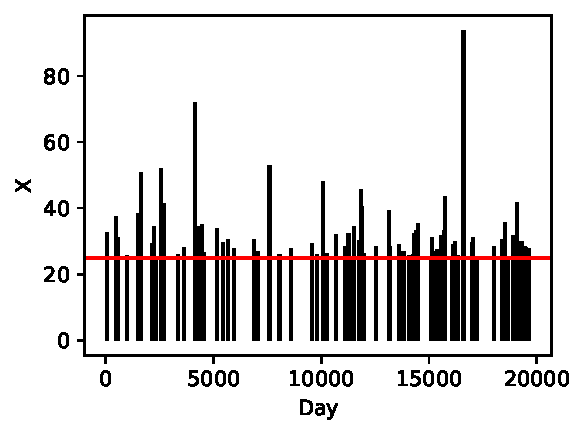
\includegraphics[width=0.49\linewidth]{plots/ppp-data.pdf}
	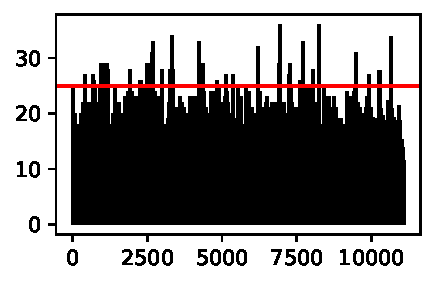
\includegraphics[width=0.49\linewidth]{plots/ws-data.pdf}
	\caption{Simulation study (left) and wind speed (right) datasets, with
		chosen thresholds in red.}
	\label{fig:data}
\end{figure}
%

%
The analyses are coded in Python, using the libraries and packages
NumPy~(\cite{numpy}), Matplotlib~(\cite{matplotlib}),
SciPy~(\cite{scipy}), and OpenTURNS~(\cite{OpenTURNS}).
The code is available on GitHub
\footnote{\url{https://github.com/tzhg/extreme-bayes}},
and consists of the files
%
\begin{enumerate}
	\item \codeword{util.py}: useful classes and functions,
	\item \codeword{priors.py}: defines the priors,
	\item \codeword{analysis-ppp.py}: analysis on simulation study,
	\item \codeword{analysis-ws.py}: analysis on real data,
	\item \codeword{jeffreys.py}: Jeffreys prior.
\end{enumerate}
%
Details of the Metropolis algorithm implementations
are tabulated in Appendix~\ref{appendix:mcmc-tables}.
%
\subsection{Simulation study}
%

%
According to the model described in \S~\ref{section:model},
the exceedances of the threshold $u$ approximately
follow a non-homogeneous Poisson point process with intensity function
%
\begin{align*}
	\lambda(x) = \frac{1}{\sigma}
		\left\{1 + \xi \left(\frac{x - \mu}{\sigma}\right)\right\}_+
		^ {-\frac{\xi + 1}{\xi}} \,,
\end{align*}
%
which is a Generalised Pareto distribution.
We simulated data for which this approximation is exact,
with known parameters.
Consistent with the study in \cite{coles1996},
we generated $19710$ observations, $n_u = 86$ of which were above
some threshold $u$. We chose $u = 25$ and $\theta = (25, 5, 0.2)$,
and set $M = n_u$, which implied that $u = \mu$.
We simulated $86$ observations from a
Generalised Pareto distribution with parameters $\theta$,
and distributed them uniformly
over the total time period of $19710$ observations,
setting the remaining observations to $0$.
%

%
The above construction of the data ensures that block maxima approximately
follow a GEV distribution whose parameters can be determined
by \eqref{eq:M-repara}.
A Q-Q plot of the fit of annual maxima is shown in Fig.~\ref{fig:ppp-qq}.
%
\begin{figure}
	\centering
	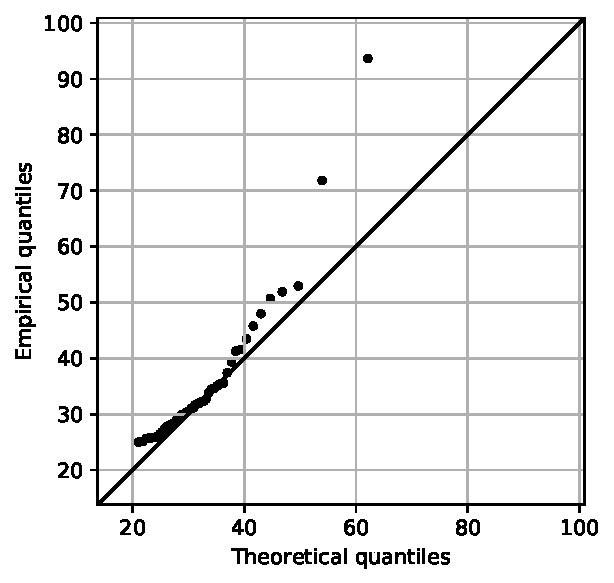
\includegraphics[width=0.55\linewidth]{plots/ppp-qq.pdf}
	\caption{Q-Q plot of GEV distribution fit for simulation study.}
	\label{fig:ppp-qq}
\end{figure}
%
The asymptotic quantiles $q_1, q_2, q_3$ were calculated
using \eqref{eq:quantile} as
%
\begin{align*}
	\hat{q}_1 = 39.211 \,,
	\quad \hat{q}_2 = 62.734 \,,
	\quad \hat{q}_3 = 99.517 \,,
\end{align*}
%
and we chose the expert specification
%
\begin{align*}
	\left(\hat{q}_1, \hat{q}_2, \hat{q}_3, 27 \right) \,.
\end{align*}
%

%
The marginals of
$\theta$ and $(q_1, q_2, q_3)$ for the different priors are illustrated
in Figs~\ref{table:ppp-theta-uni-marg} and
\ref{table:ppp-q-uni-marg}.
The posteriors of $\mu$ and $\log\sigma$ are very similar,
and very concentrated compared to the priors, whereas the
posterior of $\xi$ varies considerably,
with $k = 2$ and maximum entropy copula priors being more spread out
than $k = 3$ and independent priors.
%
\allmarginals{ppp}{simulation study}
%

%
We plotted the mean return level in Fig.~\ref{table:ppp-post-return-level}
along with 95\% credible intervals.
The black line is the asymptotic return level based on the
chosen value of $\theta$, as the block size goes to infinity.
The return levels of the $k = 2$ posteriors are almost identical,
with the maximum entropy copula posteriors
having a slightly wider credible interval.
The $k = 3$ posteriors are higher and more variable,
with the maximum entropy copula posterior
in particular having a very large credible interval.
%
\allreturnlevels{ppp}{simulation study}{%
asymptotic return level {\color{black} \textbf{(black solid)}}, }
%
\FloatBarrier
\subsection{Wind speed data}
%

%
This dataset consists of observations of average wind speed
at Tours, France over a period of $30.34$ years, from 1981 to 2011.
We restricted the data to the period November to May
to reduce non-stationarity.
Violin plots of the data are shown in Fig.~\ref{fig:ws-violinplot}.
We chose a threshold of $u = 21$ with $214$ exceedances.
The choice of threshold is investigated in \cite{coles2001},
and will not be considered here.
%
\begin{figure}
	\centering
	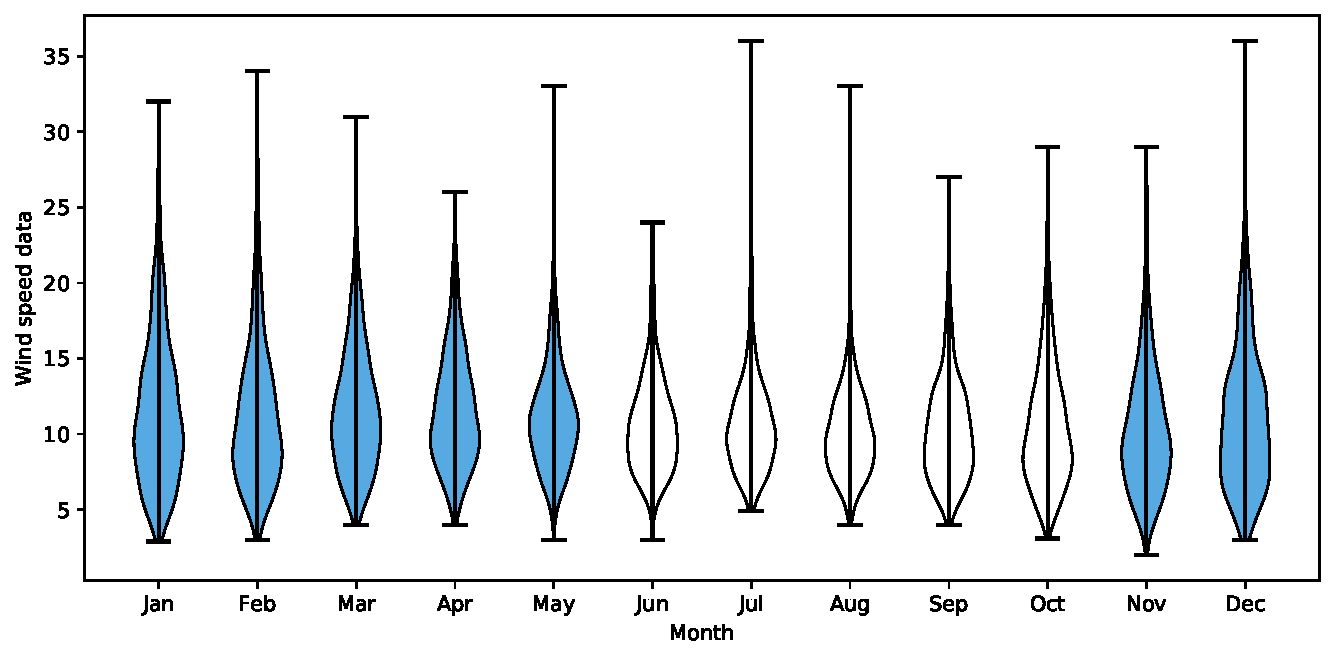
\includegraphics[width=1\linewidth]{plots/ws-boxplot.pdf}
	\caption{Violin plots of wind speed data by month.}
	\label{fig:ws-violinplot}
\end{figure}
%

%
In order to construct the priors,
we first fitted a GEV distribution on the block maxima of the data
using maximum likelihood,
with the number of blocks equal to the number of exceedances.
The fitted parameters were
$(19.065, 3.851, -0.088)$, and
a Q-Q plot of the fit is shown in Fig.~\ref{fig:ws-qq}.
%
\begin{figure}
	\centering
	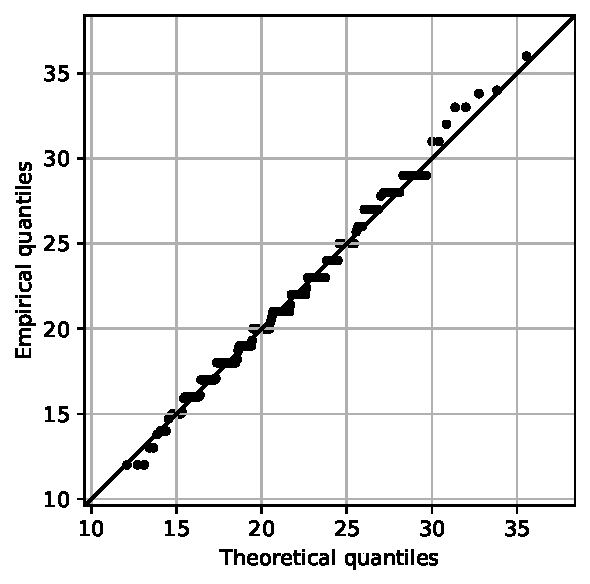
\includegraphics[width=0.55\linewidth]{plots/ws-qq.pdf}
	\caption{Q-Q plot of GEV distribution fit for wind speed data.}
	\label{fig:ws-qq}
\end{figure}
%
The quantiles $q_1, q_2, q_3$ were calculated
using \eqref{eq:quantile} as
%
\begin{align*}
	\hat{q}_1 = 26.927 \,,
	\quad \hat{q}_2 = 33.636 \,,
	\quad \hat{q}_3 = 39.004 \,.
\end{align*}
%
However, with an expert specification of
%
\begin{align*}
	\left(\hat{q}_1, \hat{q}_2, \hat{q}_3, 27 \right) \,,
\end{align*}
%
the condition \eqref{eq:C2} was not satisfied as the distributions
of the quantiles
were too close together. Therefore we chose a specification of
%
\begin{align*}
	\left(26.45, 33.636, 48, 27 \right) \,.
\end{align*}
%

%
The univariate and bivariate marginals of
$\theta$ and $(q_1, q_2, q_3)$ for the different priors are illustrated
in Figs~\ref{table:ws-theta-uni-marg} and \ref{table:ws-q-uni-marg}.
Compared to the simulation study, the posterior distribution of the
parameters $\mu$ and $\log\sigma$ are more variable,
and the
$k = 3$ maximum entropy copula is more spread out for $\log\sigma$,
and more concentrated for $\xi$.
%
\allmarginals{ws}{wind speed data}
%

%
We plotted the mean return level in Fig.~\ref{table:ws-post-return-level}
along with 95\% credible intervals. The results are similar
to the simulation study, except the return level for the
$k = 3$ maximum entropy copula posterior
is significantly higher and more variable compared
to the $k = 3$ independent copula posterior.
%
\allreturnlevels{ws}{wind speed data}{}
%
\FloatBarrier
%
\section{Discussion}
%

%
We have proposed different priors for the estimation of extreme quantiles,
and compared them on two datasets in \S~\ref{section:studies}.
%

%
Based on the results,
the choice of $k = 2$ or
$k = 3$ distributions specified is very significant
in estimating the return level.
Using $k = 3$ priors will considerably reduce the credible intervals,
at the expense of an extra distribution to specify.
Also, the use of $k = 2$ priors is unjustified as we have not yet
shown that the resulting posteriors are proper.
\cite{northrop2016} show that for least four observations,
for a uniform prior on $(\mu, \log \sigma, \xi)$,
i.e. $k = 0$, the resulting posterior is proper.
%

%
The choice of independent or maximum entropy copula is also significant.
The maximum entropy copula gives wider return level credible intervals
for the same amount of expert information provided.
As well as better taking into account the uncertainty in the model,
the greater ease of expert specification of
quantiles rather than the difference of quantiles
is a major advantage of these priors.
%

%
In order to better compare these priors,
it may be valuable to consider quantitative measures of
prior informativeness.
For example,
\cite{reimherr2014prior} derived measures
of prior sensitivity and prior informativeness
and \cite{reimherr2014prior} introduced an extension
of prior sample size to non-conjugate priors.
%
\section{Appendix}
%
\subsection{Determinants of reparametrisations of GEV model}
\label{appendix:reparametrisation}
%
\subsubsection*{Three quantile reparametrisation}
%

%
The transformation is
%
\begin{align*}
	g_3 \colon \Theta &\to \{(x, y, z) \in \R^3 \colon x < y < z\} \\
	\theta &\mapsto (q_{1}, q_{2}, q_{3}) \,,
\end{align*}
%
given by
%
\begin{align*}
	q_i = \mu + \sigma \frac{\exp(s_i \xi) - 1}{\xi} \,, \quad i = 1, 2, 3
\end{align*}
%
where $s_i \coloneqq -\log(-\log(1 - p_i))$.
We assume that
%
\begin{align*}
	p_1 < 1 - \operatorname{e} ^ {-1} \approx 0.63 \,,
\end{align*}
%
which implies that $s_i > 0$ for $i = 1, 2, 3$.
The partial derivatives are
%
\begin{align}
	\frac{\dd q_{i}}{\dd \mu}(\theta)
		&= 1 \,,
	\label{eq:q_i-derivatives-1} \\
	\frac{\dd q_{i}}{\dd \sigma}(\theta)
		&= \frac{\exp(s_i \xi) - 1}{\xi} \,,\\
	\frac{\dd q_{i}}{\dd \xi}(\theta)
		&= \frac{\sigma(s_i \xi \exp(s_i \xi)
		- \exp(s_i \xi) + 1)}{\xi ^ 2} \,,
	\label{eq:q_i-derivatives-2}
\end{align}
%
and so the determinant of the Jacobian is
%
\begin{align*}
	\det J(g_3)(\theta)
		&= \frac{\sigma}{\xi ^ {3}} \left\vert
		\begin{matrix}
			1 &1\\
			\exp(s_1 \xi)-1 &\exp(s_2 \xi)-1\\
			s_1 \xi \exp(s_1 \xi) - \exp(s_1 \xi) + 1
				&s_2 \xi \exp(s_2 \xi) - \exp(s_2 \xi) + 1
		\end{matrix}
	\right.\\
	&\qquad \qquad \left.
		\begin{matrix}
			1\\
			\exp(s_3 \xi) - 1\\
			s_3 \xi \exp(s_3 \xi) -\exp(s_3 \xi) + 1
		\end{matrix}
	\right\vert\\
	&= \frac{\sigma}{\xi ^ {3}} \abs*{
		\begin{matrix}
			1 &1 &1\\
			\exp(s_1 \xi) &\exp(s_2 \xi) &\exp(s_3 \xi)\\
			s_1 \xi \exp(s_1 \xi)
				&s_2 \xi \exp(s_2 \xi)
				&s_3 \xi \exp(s_3 \xi)
		\end{matrix} }\\	
	&= \exp\left(\xi\sum_{i = 1}^3 s_i\right) \frac{\sigma}{\xi ^ {3}}
		\abs*{
			\begin{matrix}
				\exp(-s_1 \xi) &\exp(-s_2 \xi) &\exp(-s_3 \xi)\\
				1 &1 &1 \\
				s_1 \xi 
					&s_2 \xi
					&s_3 \xi
			\end{matrix} } \\
	&= -\exp\left(\xi\sum_{i = 1}^3 s_i\right) \frac{\sigma}{\xi ^ 2}
		\abs*{
			\begin{matrix}
				1 &1 &1 \\
				\exp(-s_1 \xi) &\exp(-s_2 \xi) &\exp(-s_3 \xi) \\
				s_1 &s_2 &s_3
			\end{matrix} } \\
	&= -\exp\left(\xi\sum_{i = 1}^3 s_i\right) \frac{\sigma}{\xi ^ 2}
		(\exp(-s_2 \xi) s_3 - \exp(-s_3 \xi) s_2 \\
	&\ \phantom{=}
		+ \exp(-s_3 \xi) s_1 - \exp(-s_1 \xi) s_3 \\
	&\ \phantom{=}
		+ \exp(-s_1 \xi) s_2 - \exp(-s_2 \xi) s_1) \,.
\end{align*}
%
\subsubsection*{Two quantile reparametrisation}
%

%
The transformation is
%
\begin{align*}
	g_2 \colon \Theta &\to \R^+ \times \{(x, y) \in \R^2 \colon x < y\} \\
	\theta &\mapsto (\sigma, q_{1}, q_{2})
\end{align*}
%
given by
%
\begin{align*}
	q_i = \mu + \sigma \frac{\exp(s_i \xi) - 1}{\xi} \,, \quad i = 1, 2 \,.
\end{align*}
%
From the partial derivatives in
\eqref{eq:q_i-derivatives-1}--\eqref{eq:q_i-derivatives-2},
the determinant of the Jacobian is
%
\begin{align*}
	\det J(g_2)(\theta)
	&= \frac{\sigma}{\xi ^ 2} \abs*{
			\begin{matrix}
			0 &1 &1 \\
			1 &(\exp(s_1 \xi) - 1)\xi ^ {-1} &(\exp(s_2 \xi) - 1)\xi^{-1}  \\
			0 &s_1 \xi \exp(s_1 \xi) -\exp(s_1 \xi) + 1
				&s_2 \xi \exp(s_2 \xi) -\exp(s_2 \xi) + 1 \\
			\end{matrix} } \\
	&= \frac{\sigma}{\xi ^ 2} \abs*{
			\begin{matrix}
			&1 &1 \\
			&s_2 \xi \exp(s_2 \xi) -\exp(s_2 \xi) + 1
				&s_1 \xi \exp(s_1 \xi) -\exp(s_1 \xi) + 1 \\
			\end{matrix} } \\
	&= \frac{\sigma}{\xi ^ {2} }
		((s_1 \xi - 1) \exp(s_1 \xi) - (s_2 \xi - 1) \exp(s_2 \xi)) \,.
\end{align*}
%
\subsection{The Jeffreys prior}
\label{appendix:jeffreys}
%

%
Let $l$ be the log-likelihood of the model \eqref{eq:likelihood},
%
\begin{align*}
	l(\theta \mid \mathbf{x}) = 
		-M \left\{1 + \xi \frac{u - \mu}{\sigma}\right\}_+
		^ {-\frac{1}{\xi}} - n_u \log \sigma
		-\left(\frac{1}{\xi} + 1\right)\sum_{i = 1}^{n_u}
		\log\left\{1 + \xi\left(\frac{x_i - \mu}{\sigma}\right)\right\}_+ \,,
\end{align*}
%
and define the Fisher information matrix $I(\theta)$ with entries
%
\begin{align*}
	I(\theta)_{ij}
		= \E\left(-\frac{\partial^2 l}
		{\partial \theta_i \partial \theta_j}\right) \,.
\end{align*}
%
In the situation where we do not have access to any prior information,
\cite{jeffreys1946} proposes an uninformative prior
which is invariant to reparameterisation.
It is proportional to the square root of the determinant of the
Fisher information matrix:
%
\begin{align*}
	\pi \propto \sqrt{\det I(\phi)} \,.
\end{align*}
%
Using the Fisher information matrix derived in \cite{sharkey2017}, if we let
%
\begin{align*}
	a &\coloneqq \frac{(\xi + 1)^2}{2\xi + 1} \,, \\
	b &\coloneqq -w_1(\xi)2 v + (\xi + 1) v^2 - 1
  + 2(\xi + 1) w_1(\xi) w_2(\xi) - \xi w_4(\xi) \,, \\
	c &\coloneqq \left\{\frac{v^2}{\xi w_1(\xi)^2}
		- \frac{2\log w_1(\xi)}{\xi ^ 3}
	 + \frac{2v}{\xi ^ 2 w_1(\xi)}
	 + \frac{1}{\xi ^ 2}\left(\frac{\log w_1(\xi)}{\xi} - \frac{1}{w_1(\xi)}
		\right)^2 \right\}_+ \\
	&\ \phantom{=} + \frac{2\{\xi + \log w_1(\xi)\}_+}{M\xi ^ 3}
		- \frac{2w_2(\xi)}{\xi ^ 2w_1(\xi)}
	+ \frac{w_4(\xi)}{\xi w_1(\xi)^2} \\
	d &\coloneqq (\xi + 1)v - \xi w_3(\xi) \,, \\
	e &\coloneqq \frac{1}{\xi^2}\left\{\log w_1(\xi)
		-\frac{v \xi (\xi + 1)}{w_1(\xi)} \right\}_+ - \frac{1}{\xi + 1}
		+ \frac{w_3(\xi)}{w_1(\xi)} \,, \\
	f &\coloneqq \frac{v}{\xi ^2}\left\{\log w_1(\xi)
		+ \frac{v \xi (\xi + 1)}{w_1(\xi)} \right\}_+	
		- w_2(\xi) + \frac{w_4(\xi)}{w_1(\xi)} \,,
\end{align*}
%
where
%
\begin{align*}
	v &\coloneqq \frac{u - \mu}{\sigma} \,, \\
	w_1(\xi) &\coloneqq \{1 + \xi v\}_+ \,, \\
	w_2(\xi) &\coloneqq \frac{\{1 + (\xi + 1) v\}_+}{\xi + 1} \,, \\
	w_3(\xi) &\coloneqq \frac{\{1 + (2\xi + 1) v\}_+}{2\xi + 1} \,, \\
	w_4(\xi) &\coloneqq \frac{\{(2\xi + 1)(\xi + 1) v^2 
		+ 2(2\xi + 1) v + 2\}_+}{2\xi + 1} \,,
\end{align*}
%
then Jeffreys prior is proportional to
%
\begin{align*}
	\pi(\theta) \propto
	 \frac{\sqrt{a(df-e^2) + b(ce-bf) + c(be-dc)}}
		{\sigma^2 w_1(\xi)^2} \,.
\end{align*}
%
Fig.~\ref{fig:jeffreys} shows the Jeffreys prior as a function of $\xi$,
with $(\mu, \sigma) = (0,  1)$, $u = \mu$, and $M = 1$.
%
\begin{figure}
	\centering
	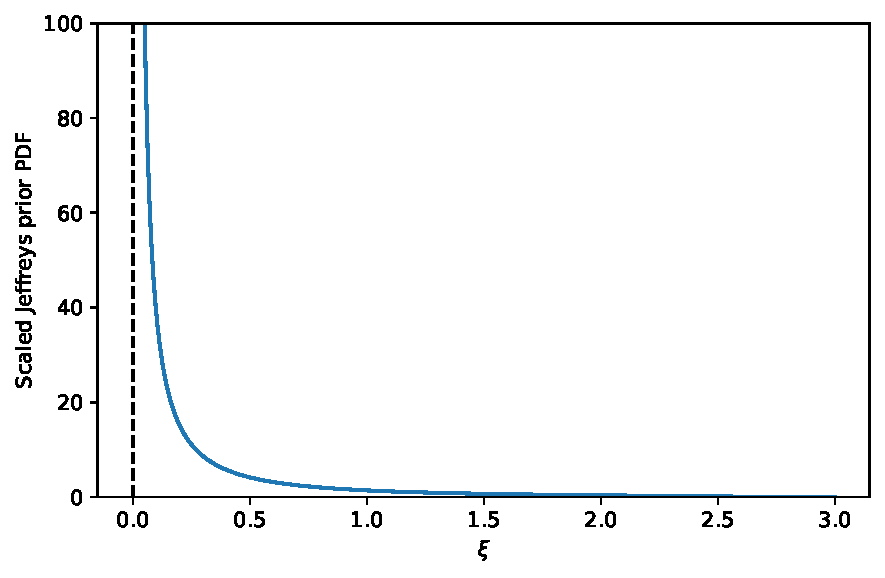
\includegraphics[width=0.7\linewidth]{plots/jeffreys.pdf}
	\caption{Scaled Jeffreys prior PDF against $\xi$.}
	\label{fig:jeffreys}
\end{figure}
%
\subsection{Maximum entropy copula: condition on marginals}
\label{appendix:C2}
%

%
The construction of the maximum entropy distribution in
\S~\ref{section:order} requires the following condition on the marginals:
for a sequence of distributions $(F_i)_{1 \geq i \geq d}$,
%
\begin{align}
	\forall 1 \leq i \leq d - 1
		\ \forall x \in \{x \colon 1 > F_i(x), F_{i + 1}(x) > 0\}
		\ (F_i(x) > F_{i + 1}(x))\,.
	\label{eq:C2-2}
\end{align}
%
We will investigate this condition for
Weibull and gamma distributed marginals.
%
\subsubsection*{Weibull distribution}
%
Let $1 \leq i \leq d - 1$. If the marginals are Weibull distributed,
then we have that
%
\begin{align*}
	1 > F_i(x), F_{i + 1}(x) > 0 \iff x > 0 \,.
\end{align*}
%
The CDF when $x > 0$ is
%
\begin{align*}
	F_i(x) = 1 - \exp\left(-\left(\frac{x}{\lambda_i}\right)
		^ {k_i}\right) \,,
\end{align*}
%
with $k_i$, $\lambda_i > 0$. Let $x > 0$.
Then \eqref{eq:C2-2} is equivalent to
%
\begin{align*}
	1 - \exp\left(-\left(\frac{x}{\lambda_i}\right)
		^ {k_i}\right) &> 1- \exp\left(-\left(\frac{x}{\lambda_{i + 1}}\right)
		^ {k_{i + 1}}\right)\\
	\iff \left(\frac{x}{\lambda_i}\right) ^ {k_i} &>
		\left(\frac{x}{\lambda_{i + 1}}\right) ^ {k_{i + 1}} \,.
\end{align*}
%
If $k_i = k_{i + 1} = k$,
%
\begin{align*}
	\left(\frac{x}{\lambda_i}\right) ^ k
		> \left(\frac{x}{\lambda_{i + 1}}\right) ^ k&
		\iff \frac{x}{\lambda_i} > \frac{x}{\lambda_{i + 1}}\\
	&\iff \frac{1}{\lambda_i} > \frac{1}{\lambda_{i + 1}}\\
	&\iff \lambda_i < \lambda_{i + 1} \,.
\end{align*}
%
If $k_i \neq k_{i + 1}$,
%
\begin{align*}
	F_i(x) =F_{i + 1}(x)
		&\iff \left(\frac{x}{\lambda_i}\right) ^ {k_i}
		= \left(\frac{x}{\lambda_{i + 1}}\right) ^ {k_{i + 1}}\\
	&\iff \exp\left(k_i (\log x - \log\lambda_i)\right)
		=\exp\left({k_{i + 1}}(\log x - \log\lambda_{i + 1})\right)\\
	&\iff k_i (\log x - \log\lambda_i)
		= {k_{i + 1}} (\log x - \log\lambda_{i + 1})\\
	&\iff k_i \log x - k_i \log\lambda_i 
		= {k_{i + 1}} \log x - {k_{i + 1}} \log\lambda_{i + 1}\\
	&\iff k_i \log x - {k_{i + 1}} \log x
		=k_i \log\lambda_i - {k_{i + 1}} \log\lambda_{i + 1}\\
	&\iff (k_i - {k_{i + 1}}) \log x 
		= k_i \log\lambda_i - {k_{i + 1}} \log\lambda_{i + 1}\\
	&\iff \log x
		= \frac{k_i \log\lambda_i - {k_{i + 1}}
		\log\lambda_{i + 1}}{k_i - {k_{i + 1}}}\\
	&\iff x
		= \exp\underbrace{\left(\frac{k_i \log\lambda_i - {k_{i + 1}}
		\log\lambda_{i + 1}}{k_i - {k_{i + 1}}}\right)}
		_{\eqqcolon h(k_i, \lambda_i, k_{i + 1}, \lambda_{i + 1})} \,.
\end{align*}
%
Therefore the two CDFs intersect, and so \eqref{eq:C2-2} cannot be satisfied.
In conclusion, the condition is equivalent to
%
\begin{align*}
	(k_i = k_{i + 1}) \land (\lambda_i < \lambda_{i + 1})
		\quad \forall 1 \leq i \leq d - 1 \,.
\end{align*}
%

%
In practice however, as
$y \coloneqq h(k_i, \lambda_i, k_{i+1}, \lambda_{i+1}) \to \pm \infty$,
the intersection will tend to the bounds of the set
$\{x \colon 1 > F_i(x), F_{i + 1}(x) > 0\}$ and so \eqref{eq:C2-2}
will be asymptotically satisfied. When does this happen?
Consider a reparametrisation
%
\begin{align*}
	(k_i, \lambda_i, k_{i + 1}, \lambda_{i + 1}) \mapsto
		(k_i, \lambda_i, k_i - {k_{i + 1}}, \lambda_{i + 1}) \,,
\end{align*}
%
which implies that
%
\begin{align*}
	h(k_i, \lambda_i, z_{i}, \lambda_{i+1})
		=\frac{k_i \log\lambda_i + {(z_{i} - k_{i})}
		\log\lambda_{i + 1}}{z_{i}} \,,
		\quad z_{i} < k_i,\ z_{i} \neq 0 \,.
\end{align*}
%
Then
%
\begin{itemize}
	\item As $z_i \to 0$, $y \to +\infty$,
	\item As $k_i \to +\infty$, $y \to \pm\infty$, with sign depending
		on the sign of $\log(\frac{\lambda_i}{\lambda_{i + 1}})$,
	\item As $\lambda_i \to +\infty$ or $\lambda_{i + 1} \to 0$,
		$y \to +\infty$,
	\item As $\lambda_i \to 0$ or  $\lambda_{i + 1}\to +\infty$,
		$y \to -\infty$.
\end{itemize}
%
\subsubsection*{Gamma distribution}
%

%
Let $1 \leq i \leq d - 1$.
If the marginals are gamma distributed, then we have that
%
\begin{align*}
	1 > F_i(x), F_{i+1}(x) > 0 \iff x > 0 \,.
\end{align*}
%
Suppose that $x > 0$, and that we have two such distributions,
%
\begin{align*}
	F_1 \sim \Gamma(\alpha_1, \beta_1) \quad \text{and} \quad
	F_2 \sim \Gamma(\alpha_2, \beta_2) \,,
\end{align*}
%
with PDFs $f_1$ and $f_2$ given by
%
\begin{align*}
	f_i(x) = \frac{\beta_i ^ {\alpha_i} x ^ {\alpha_i - 1}
		\exp(-\beta_i x)}{\Gamma(\alpha_i)} \quad  i = 1, 2 \,.
\end{align*}
%
Let $x > 0$, and define
%
\begin{align*}
	\phi(x) = F_2(x) - F_1(x) \,,
\end{align*}
%
so that if $(i, i + 1) = (1, 2)$,
\eqref{eq:C2-2} is equivalent to $\phi(x) < 0$,
and if $(i, i + 1) = (2, 1)$,
\eqref{eq:C2-2} is equivalent to $\phi(x) > 0$.
%
We have that
%
\begin{align*}
	\phi'(x) &= f_2(x) - f_1(x)\\
	&= f_1(x) \left(\frac{f_2(x)}{f_1(x)} - 1\right)\\
	&= f_1(x) \left(\frac{\Gamma(\alpha_1)\beta ^ {\alpha_2}_2}
		{\Gamma(\alpha_2)\beta ^ {\alpha_1}_1} x^{\alpha_2 - \alpha_1}
		\exp((\beta_1 - \beta_2) x) - 1\right) \,.
\end{align*}
%
Let
%
\begin{align*}
	C \coloneqq \frac{\Gamma(\alpha_1) \beta ^ {\alpha_2}_2}
		{\Gamma(\alpha_2) \beta ^ {\alpha_1}_1} > 0
\end{align*}
%
and
%
\begin{align*}
	f(x) \coloneqq C x ^ {\alpha_2 - \alpha_1}
		\exp((\beta_1 - \beta_2) x) - 1 \,.
\end{align*}
%
Then
%
\begin{align*}
	f'(x) &= C\left[(\alpha_2 - \alpha_1) x ^ {\alpha_2 - \alpha_1 - 1}
		\exp((\beta_1 - \beta_2) x) + x ^ {\alpha_2 - \alpha_1}
		\exp((\beta_1 - \beta_2) x)(\beta_1 - \beta_2) \right]\\
	&=\underbrace{C x ^ {\alpha_2 - \alpha_1 - 1} \exp((\beta_1 - \beta_2) x)}
		_{ > 0} \left[(\alpha_2 - \alpha_1) + x (\beta_1 - \beta_2)\right]
\end{align*}
%
\subsubsection*{\underline{Case 1:
	$(\alpha_1 \leq \alpha_2 \land \beta_1 \geq \beta_2)
	\land \neg (\alpha_1 = \alpha_2 \land \beta_1 = \beta_2)$}}

%
We have that $\alpha_2 - \alpha_1 \geq 0$ and
$\beta_1 - \beta_2 \geq 0$, and therefore
%
\begin{align*}
	(\alpha_2 - \alpha_1) + x(\beta_1 - \beta_2) &> 0\\
	\implies f'(x) & > 0 \,.
\end{align*}
%
This implies that $f$ is strictly increasing on $\R^+$.
%
\begin{enumerate}
	\item If $\alpha_1 < \alpha_2$, we have that
		\begin{align*}
			\lim_{x \to 0^+} f(x) = -1 \quad \text{and} \quad
				\lim_{x \to +\infty} f(x) = +\infty\,.
		\end{align*}
	\item If $\alpha_1 = \alpha_2 = \alpha$ and $\beta_1 > \beta_2$,
		we have that
		\begin{align*}
			\lim_{x \to 0^+} f(x)
				= \left(\frac{\beta_2}{\beta_1}\right) ^ \alpha - 1 < 0 \quad
				\text{and} \quad \lim_{x \to +\infty} f(x) = +\infty \,.
		\end{align*}
\end{enumerate}
%
Therefore in both cases, there exists a unique $z_0 > 0$
such that $f(z_0) = 0$. This implies that
%
\begin{align*}
	\begin{cases}
		\phi'(x) < 0 &\text{if} \quad x < z_0 \,,\\
		\phi'(x) = 0 &\text{if} \quad x = z_0 \,,\\
		\phi'(x) > 0 &\text{if} \quad x > z_0 \,.
	\end{cases}
\end{align*}
%
In order to proceed we will need the following Lemma.
%
\begin{lemma}
	\begin{enumerate}
		\item Let $f \colon (a, b] \to \R$ be continuous on $(a, b]$
			and differentiable on $(a, b)$, with 
			$a \in \R \cup \{+\infty\}, b \in \R$. If for all $x \in (a, b)$,
			\ $f'(x) > 0$ (resp. $<$) and $\lim_{x \to a^+} f(x) = L \in \R$,
			then for all $z \in (a, b]$, $f(z) > L$ (resp. $<$).
		\item Let $f \colon [a, b) \to \R$ be continuous on $[a, b)$
			and differentiable on $(a, b)$, with
			$a \in \R, b \in \R \cup \{+\infty\}$. If for all $x\in(a, b)$,
			\ $f'(x) > 0$ (resp. $<$) and $\lim_{x \to b^-} f(x) = L \in \R$,
			then for all $z \in [a, b)$, $f(z) < L$ (resp. $>$).
	\end{enumerate}
	\label{lemma:limit}
\end{lemma}
%
\begin{proof}
	We will prove the first case, for $f'(x) > 0$,
	as both cases are symmetrical. Suppose that $z \in (a, b)$.
	We need to show that $f(z),f(b) > L$. Let $y \in (a, z)$.
	As $f'$ is strictly positive on $(a, b)$, $f$ is strictly increasing
	(by the mean value theorem), and so $f(z) - f(y) = c > 0$.
	Therefore $f(z) > f(y) + \frac{c}{2}$.
	Then $f(z) = \lim_{y \to a^+} f(z) \geq \lim_{y \to a^+} f(y)
	+ \frac{c}{2} = L + \frac{c}{2} > L$.
	Furthermore, $f(b) = \lim_{z \to b^-} f(z) \geq \lim_{x \to b^-} 
	(L + \frac{c}{2}) = L + \frac{c}{2} > L$.
\end{proof}
%

%
By Lemma~\ref{lemma:limit}, for all $z \in (0, z_0]$,
$\phi(z) < \lim_{x\to 0^+}\phi(x)=0$, and for all $z \in[z_0, +\infty)$,
$\phi(z) < \lim_{x \to +\infty} \phi(x) = 0$.
Therefore for all $x > 0$, $\phi(x) < 0$, and so if $(i, i + 1)=(1, 2)$,
\eqref{eq:C2-2} is satisfied, and if $(i, i + 1) = (2, 1)$,
\eqref{eq:C2-2} is violated.
%
\subsubsection*{\underline{Case 2: $\alpha_1 < \alpha_2, \  \beta_1 < \beta_2$}}
%

%
Since
%
\begin{align*}
	\lim_{x \to 0^+} f(x) = -1 \,,
\end{align*}
%
there exists a $\delta > 0$ such that for all $z \in (0, \delta]$,
$f(z) = \phi'(z) < 0$, and so by Lemma~\ref{lemma:limit},
$\phi(z) < \lim_{x \to 0^+} \phi(x) = 0$. Since
%
\begin{align*}
	\lim_{x \to +\infty} f(x) = -1 \,,
\end{align*}
%
there exists a $\delta' > 0$ such that for all $z \in [\delta', +\infty)$,
$f(z) = \phi'(z) < 0$, and so by Lemma~\ref{lemma:limit},
$\phi(z) > \lim_{x \to 0^+} \phi(x) = 0$.
Therefore $\phi$ is neither strictly positive nor strictly negative,
and so if either $(i, i + 1) = (1, 2)$ or
$(i, i + 1) = (2, 1)$, \eqref{eq:C2-2} is violated.
%

%
In conclusion, we have shown that the condition is equivalent to
%
\begin{align*}
	(\alpha_i \leq \alpha_{i + 1} \land \beta_{i}
	\geq \beta_{i + 1}) \land \neg(\alpha_i = \alpha_{i+1} \land \beta_i
	= \beta_{i + 1}) \quad \forall 1 \leq i\leq d - 1 \,.
\end{align*}
%
Like in the Weibull case, the condition can be asymptotically satisfied.
For instance, if the means $\frac{\alpha}{\beta}$ are sufficiently separated,
and the variances $\frac{\alpha}{\beta ^ 2}$ are small,
there will be less significant overlap between the CDFs.
%
\subsection{Obtaining truncated normal parameters from mean and variance}
\label{appendix:tn-invert}
%

%
Suppose that we are given the mean $\mu^*$ and variance $(\sigma^*) ^ 2$
of a random variable $X$ which follows a truncated normal distribution
with support parameters $a = 0$ and $b = +\infty$,
and we would like to determine the remaining parameters $\mu$ and $\sigma$.

%
This means that we need to invert the equations for the mean and variance,
given by~(\cite{johnson})
%
\begin{align*}
	\E(X) &= \mu + \frac{\phi(\alpha)}{1 - \Phi(\alpha)} \sigma \\
	\Var(X) &= \sigma ^ 2
		\left(1 + \frac{\alpha \phi(\alpha)}{1 - \Phi(\alpha)}
		- \left(\frac{\phi(\alpha)}{1 - \Phi(\alpha)}\right) ^ 2\right) \,,
\end{align*}
%
where $\phi$ and $\Phi$ are the PDF and CDF of the
standard normal distribution respectively and
%
\begin{align}
	\alpha \coloneqq -\frac{\mu}{\sigma} \,.
	\label{tn-alpha}
\end{align}
%
Setting
%
\begin{align*}
	H(x) \coloneqq \frac{\phi(x)}{1 - \Phi(x)} \,,
\end{align*}
%
which is the hazard function of the standard normal distribution, we can
simplify the equations to
%
\begin{align}
	\E(X) &= \mu + H(\alpha)\sigma \label{tn-mean} \\
	\Var(X) &= \sigma ^ 2 \left(1 + \alpha H(\alpha)
		- (H(\alpha)) ^ 2 \right)
		\label{tn-var} \,.
\end{align}
%
Therefore,
%
\begin{align*}
	\left(\frac{\sigma^*}{\mu^*}\right)^2 &=
		\frac{\sigma ^ 2 \left(1 + \alpha H(\alpha)
		- (H(\alpha)) ^ 2 \right)}{%
		\left(\mu + H(\alpha) \sigma\right) ^ 2} \\
	&= \frac{1 + \alpha H(\alpha) - (H(\alpha)) ^ 2}
		{\left(H(\alpha) - \alpha\right) ^ 2} \eqqcolon f(\alpha) \,, \\
\end{align*}
%
and once we have $\alpha$, from \eqref{tn-mean} we have
%
\begin{align*}
	\frac{\mu^*}{\sigma} = H(\alpha) - \alpha
		\implies \sigma = \frac{\mu^*}{H(\alpha) - \alpha}
\end{align*}
%
and from \eqref{tn-alpha},
%
\begin{align*}
	\alpha = -\frac{\mu}{\sigma} \implies \sigma =  -\alpha \mu \,.
\end{align*}
%
It remains to solve $f(\alpha) = \left(\frac{\sigma^*}{\mu^*}\right) ^ 2$.
This can be done numerically using
Newton's method with the derivative of $f$.
Since
%
\begin{align*}
	\phi'(x) = -x \phi(x) \,,
\end{align*}
%
the derivative of $H$ is
%
\begin{align*}
	H'(x) &= \frac{(1 - \Phi(x)) x (-\phi(x))
		- \phi(x)(- \phi(x))}{(1 - \Phi(x))^2} \\
	&= \phi(x) \frac{-(1 - \Phi(x)) x + \phi(x)}
		{(1 - \Phi(x))^2} \\
	&= H(x) \frac{-(1 - \Phi(x)) x + \phi(x)}
		{1 - \Phi(x)} \\
	&= H(x) \left(\frac{-(1 - \Phi(x)) x}
		{1 - \Phi(x)} + H(x) \right) \\
	&= H(x) \left(H(x) - x \right) \,.
\end{align*}
%
Therefore the derivative of $f$ is
%
\begin{align*}
	f'(x) &= \left(\left(H(x) - x\right) ^ 2
		\left(H(x) + x H(x) \left(H(x) - x \right)
		- 2 (H(x)) ^ 2 \left(H(x) - x \right)\right)\right. \\
	&\ \phantom{=} \left. - \left(1 + x H(x) - (H(x)) ^ 2\right)
		2 \left(H(x) - x\right)
		\left(H(x) \left(H(x) - x \right) - 1\right)\right)
		\left(H(x) - x\right) ^ {-4} \\
	&= \frac{(2 + H(x) (H(x) - x) (-3 + (H(x) - x) x))}{(H(x) - x) ^ 3} \,.
\end{align*}
%
\subsection{Spike-and-slab prior distribution for \boldmath$\xi$}
\label{appendix:prior-ss}
%

%
This is a prior with a non-zero probability mass (spike) at $\xi = 0$,
and a flat slab elsewhere.
%

%
We use the method proposed by \cite{kuo1998}.
We introduce an indicator random variable $\gamma$ such that
$\gamma = 0$ when $\xi$ is ``in'' the spike
and $\gamma = 1$ when $\xi$ is ``in'' the slab.
The probability that $\xi$ is non-zero can then be calculated
as the expectation of $\gamma$.
We also need a random variable $\beta$ such that $\xi = \beta \gamma$,
which determines the distribution of $\xi$ in the slab.
Our model now has parameters $\eta \coloneqq (\mu, \sigma, \beta, \gamma)$,
and we suppose that $\gamma$ does not depend on the other parameters.
%

%
If we have a prior $\pi_\theta$ for $\theta$, then we can set
%
\begin{align*}
	\pi_{\mu, \sigma, \beta} &\coloneqq \pi_\theta \\
	\pi_\gamma(\gamma)
		&\coloneqq \alpha ^ \gamma (1 - \alpha) ^ {1 - \gamma} \\
	\implies \pi_{\eta}(\eta)
		&= \pi_\theta(\mu, \sigma, \beta)
		\alpha ^ \gamma (1 - \alpha) ^ {1 - \gamma} \,,
\end{align*}
%
with $\alpha \in [0, 1]$. The posterior is then proportional to
%
\begin{align*}
	\pi_{\eta \mid \mathbf{x}}(\eta \mid \mathbf{x}) &\propto
		L(\mu, \sigma, \beta \gamma \mid \mathbf{x})
		\pi_\theta(\mu, \sigma, \beta)
		\alpha ^ \gamma (1 - \alpha) ^ {1 - \gamma} \,.
\end{align*}
%

%
Since, up to the same constant of proportionality, we have
%
\begin{align*}
	\pi_{\gamma \mid \mu, \sigma, \beta, \mathbf{x}}
		(0 \mid \mu, \sigma, \beta, \mathbf{x}) &\propto
		(1 - \alpha) L(\mu, \sigma, 0 \mid \mathbf{x})
\end{align*}
and
\begin{align*}
	\pi_{\gamma \mid \mu, \sigma, \beta, \mathbf{x}}
		(1 \mid \mu, \sigma, \beta, \mathbf{x}) &\propto
		\alpha L(\mu, \sigma, \beta \mid \mathbf{x}) \,,
\end{align*}
%
the full conditional of $\gamma$ is a Bernoulli distribution
with probability of success
%
\begin{align*}
	\frac{\alpha L(\mu, \sigma, \beta \mid \mathbf{x})}
		{\alpha L(\mu, \sigma, \beta \mid \mathbf{x})
		+ (1 - \alpha) L(\mu, \sigma, 0 \mid \mathbf{x})} \,.
\end{align*}
%
We can sample $\gamma$ from its full conditional
in the Metropolis–Hastings algorithm.
%
\subsection{Metropolis-Hastings algorithm implementation details}
\label{appendix:mcmc-tables}
%

%
In Tables~\ref{table:ppp-i-1}--\ref{table:ws-me-2},
we show details on our
implementations of the Metropolis-Hastings algorithm, including
the proposal distributions, initialisation, sample size, traceplots,
histograms, and acceptance rates.
%
\metroall{ppp}{simulation study}
\metroall{ws}{wind speed data}
%
\FloatBarrier
\printbibliography
%
\end{document}